\documentclass[../main.tex]{subfiles}
\graphicspath{{\subfix{../images/}}}

\begin{document}
As it turns out, there's more to algebra than pure uninspiring symbol pushing. In this chapter we look at some structures and concepts in elementary algebra.

\begin{figure}[H]
    \centering
    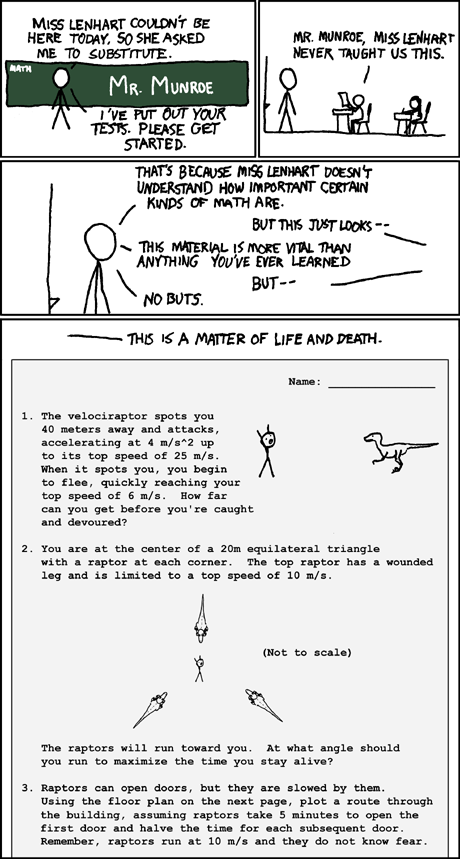
\includegraphics[scale=0.5]{xkcd_substitute.png}
    \caption{Comic from https://xkcd.wtf/135/}
\end{figure}

\subsection{A Buffet Spread}
Our first problem showcases a powerful proving technique: proof by contradiction.
\begin{example}[Classic]
Let $a, b$ be integers. We say that an integer is \textit{tasty} if it is expressible in the form $a^2+ab+b^2$. Prove that 2 is not tasty.
\end{example}
Classically, $a^2+ab+b^2$ is a so-called quadratic form. This suggests a direct proof is not feasible: enter the realm of contradictions.

\begin{proof}
We first suppose for the sake of contradiction that $2$ is expressible in this form. Then we have, for some $a,b$: 
$$a^2+ab+b^2=2 \Longrightarrow (2a+b)^2+3b^2=8.$$

Now, the problem falls to simple casework: neither $b^2=0$, $b^2=1$ nor $b^2=4$ is possible, but we assumed initially that $2$ is tasty! Since a wrong assumption resulted in an absurd conclusion, this means that our initial assumption must be wrong. In other words, $2$ is not tasty.
\end{proof}
\begin{moral}
The hardest part is to realise that a direct approach may be difficult...
\end{moral}
This question is really a test of fundamentals: in essence, the number theory starter leads to an algebra finish.
\begin{example}[2021 H3 Math P1 Q4]
Let $a,b,c,d$ be positive integers such that
\begin{equation}\label{5.3-det}
    (ad-bc)^2=(a+b)(c+d)
\end{equation}
Show that there exists coprime positive $x,y$ and a positive integer $z$ such that
$$a+b=x^2z, c+d=y^2z.$$
\end{example}
Here, we say that two integers $r,s$ are \textbf{coprime} (or \textbf{relatively prime}) \textit{if and only if} $\gcd(r,s)=1$, meaning that their greatest common factor is $1$. The readers more familiar with number theory will quickly recall that the problem implies that $\gcd(a+b, c+d)=z$.

Indeed, we may claim as such, since the problem only asks of us to prove the existence of \textit{a} positive integer $z$. We begin by defining $z=\gcd(a+b, c+d)$, whence $a+b=mz$, $c+d=nz$ for some coprime $m, n$. Our goal is now to show that $m$ and $n$ are both perfect squares.

From \eqref{5.3-det}, $(ad-bc)^2=mnz^2$, so $mn$ is a perfect square. Now, consider the prime decompositions:
    $$m = \prod {p_i}^{e_i}, \;n = \prod {q_j}^{f_j}$$
Since $m$ and $n$ are coprime, no $p_i$ and $q_j$ are equal.
Moreover,
$$mn = {p_1}^{e_1}\cdot{p_2}^{e_2}\cdots{q_1}^{f_1}\cdot{q_2}^{f_2}\cdots.$$
Since $mn$ is a perfect square, all $e_i$ and $f_j$ are even, which implies that $m$ and $n$ are both perfect squares.

Now, we may write $m=x^2$, $n=y^2$ for some coprime $x,y$ since $m, n$ are coprime. Plugging this back into our original definition, we have $a+b=x^2z, c+d=y^2z$, as required.

\begin{example}[cont.]
Find a quadratic equation that $\frac{y}{x}$ satisfies, and hence prove that $4ac+1$ is a perfect square.
\end{example}
\begin{remark}
At face value, this question says that for a matrix $M=\begin{pmatrix} a&b\\c&d
\end{pmatrix}$ with integer entries, if the square of it's determinant is the product of the sum of it's diagonals, then $4ac+1$ is a perfect square. As it stands, I don't know of any approach that involves this idea.
\end{remark}
We have
$$\frac{y^2}{x^2}=\frac{c+d}{a+b}.$$
Square-rooting this term is slightly obstructive, so we should find another way to express $\frac{y}{x}$. Since we have not used $\eqref{5.3-det}$, this might be the time. Dividing across by $(a+b)^2$ (since it is non-zero), we have
$$\frac{(ad-bc)^2}{(a+b)^2}=\frac{c+d}{a+b}=\frac{y^2}{x^2} \Longrightarrow \frac{ad-bc}{a+b}=\frac{y}{x}$$
since $\frac{y}{x}$ is positive.

Our quadratic is
\begin{align*}
   &\frac{py^2}{x^2}+\frac{qy}{x}+r=\frac{p(c+d)}{a+b}+\frac{q(ad-bc)}{a+b}+r=0 \\
   \Longleftrightarrow &p(c+d)+q(ad-bc)+r(a+b)=0
\end{align*}

This means we should make a choice for $p, q$ and $r$. Let us investigate this observation: if we choose $p=a, r=-c$,
\begin{align*}
    a(c+d)+q(ad-bc)-c(a+b)&=ac+ad+q(ad-bc)-ac-bc\\
    &=ad+q(ad-bc)-bc=0,
\end{align*}
almost as if it's forcing $q=-1$!
Thus, a possible quadratic equation is $au^2-u-c=0$ with $u=\frac{y}{x}$.

Now, if $x$ is a rational root, then we realise that $\Delta$ needs to be a rational square, that is the square of a rational number, and that this condition also implies that $x$ is a rational root. We say that this bi-directional relationship is a \textbf{necessary and sufficient} condition. In this problem, $\frac{y}{x}$ is a rational root to our quadratic, so $4ac+1$ is a rational square. However, $4ac+1$ is also a positive integer, and so it must be a perfect square!

As again, proofs should be written in the forwards direction, and we present so succinctly.
\begin{proof}
I claim that the quadratic equation is $au^2-u-c=0$ if $ad-bc > 0$ and $au^2+u-c=0$ if $ad-bc < 0$.

We have $$\frac{y^2}{x^2}=\frac{c+d}{a+b}, \; \frac{y}{x}=\frac{ad-bc}{a+b},$$
Thus, $$\frac{a(c+d)}{a+b}-\frac{ad-bc}{a+b}-c=\frac{a(c+d)-(ad-bc)-c(a+b)}{a+b}=0.$$

The discriminant is $\Delta=4ac+1$. Since $\frac{y}{x}$ is a rational root, $\Delta$ is a rational square. Moreover, $4ac+1$ is a positive integer, and so it is a perfect square.
\end{proof}
\begin{moral}
The main challenge was discovering the quadratic equation, but we are motivated by the term $4ac+1$, which reminded us of the quadratic discriminant. Finally, the treatment of $\Delta$ required us to recall the definition of the discriminant and to argue that it must be a rational square, which implied that it is also a perfect square given that $a,b,c,d$ are all integers.
\end{moral}

Armed with the problem above, we use the idea of divisibility to motivate an approach to the following problem.
\begin{example}[USAMO 2015 P1, JMO P2]
Solve in integers the equation
$$x^2+xy+y^2=\left(\frac{x+y}{3}+1\right)^3.$$
\end{example}
To start off, we know LHS is an integer and so RHS must also be an integer. This means $\frac{x+y}{3}$ is also an integer, so we are motivated to write $x+y=3k$ for some integer $k$.

On the other hand, LHS contains a pesky $xy$ term. Here comes the \textit{trick}: to kill off this nasty term, we rely on the symmetry of $x$ and $y$. Consider $a=x+y, b=x-y$:
    $$xy= \frac{(a+b)(a-b)}{4}\;x^2+y^2= \frac{(a+b)^2+(a-b)^2}{4}$$
and the equation becomes
$$\frac{1}{4}\left((a+b)^2+(a+b)(a-b)+(a-b)^2\right)=\left(\frac{a}{3}+1\right)^3 \Longrightarrow 3a^2+b^2=4\left(\frac{a}{3}+1\right)^3.$$
Letting $a=3k$, $27k^2+b^2=4(k+1)^3 \Longrightarrow b^2=4k^3-15k^2+12k+4$.
At this point, surely the cubic must factor. Indeed, we miraculously see
$$b^2=(k-2)^2(4k+1) \Longrightarrow 4k+1=m^2,$$
for odd $m$ (see the problem above for a similar reasoning).

Now, we are done, since by backsubstituting, we have:
$$a=3k=\frac{3}{4}(m^2-1), \quad b^2=(k-2)^2(4k+1)=\left(\frac{m^2-9}{4}\right)^2m^2 \Longrightarrow b=\pm \frac{m^3-9m}{4}.$$
Hence,
$$x=\frac{1}{8}\left(3(m^2-1)\pm(m^3-9m)\right)\quad\text{and}\quad y=\frac{1}{8}\left(3(m^2-1)\mp(m^3-9m)\right).$$

Is that all? Not quite! Don't forget that we are told to solve the given equation over the integers, so we should show also that our solutions are indeed all integers. Fortunately, since $m$ is odd, we may let $m=2n+1$ so that
$$\boxed{x=n^3+3n^2-1\quad\text{and}\quad y=-n^3+3n+1},$$
and permutations (note that the equation is symmetric in $x$ and $y$!).
\begin{moral}
A poster child for "keeping it simple".
\end{moral}

Finally, we end off with an example on induction, and the direction of mathematical logic.
\begin{example}[2021 H2 Further Math P1 Q4]
For real $x$ and any positive integer $n$, the function $F_n$ is defined by
$$F_n(x)=\frac{x(x+1)(x+2)\cdots(x+n-1)}{n!}.$$
Prove by induction that, for all positive integers $n$, $F_n\left(\frac{1}{2}\right) < \frac{1}{\sqrt{2n+1}}$.
\end{example}
The base case is simple to deal with, so we focus on the inductive hypothesis first. For the moment, write $x=\frac{1}{2}$ and assume that $F_k(x)<\frac{1}{\sqrt{2k+1}}$.

For $F_{k+1}(x)$, we have
\begin{align*}
    F_{k+1}(x)&=\frac{x(x+1)(x+2)\cdots(x+k-1)}{k!} \cdot \frac{x+k}{k+1} \\
    &< \frac{1}{\sqrt{2k+1}} \cdot \frac{2k+1}{2(k+1)} \\
    &= \frac{2k+1}{2(k+1)\sqrt{2k+1}} \\
\end{align*}
How do we proceed? To start, we know that $\frac{2k+1}{2(k+1)} < 1$, but that gives $F_{k+1}(x) < \frac{1}{\sqrt{2k+1}}$, no good. On the other hand, our required form is $F_{k+1}(x) < \frac{1}{\sqrt{2k+3}}$, so we may be tempted to claim $\frac{1}{\sqrt{2k+1}} < \frac{1}{\sqrt{2k+3}}$, but this is not true. Just try $k=1$!

To this end, we try the most brain-dead thing possible: we want $F_{k+1}(x) < \frac{1}{\sqrt{2k+3}}$, so it would be great if we have $\frac{2k+1}{2(k+1)\sqrt{2k+1}}<\frac{1}{\sqrt{2k+3}}$. Trying our luck:
\begin{align*}
    &\frac{2k+1}{2(k+1)\sqrt{2k+1}} < \frac{1}{\sqrt{2k+3}} \\
    \Longleftrightarrow& (2k+1)\sqrt{2k+3} < 2(k+1)\sqrt{2k+1} && \parbox{5.5cm}{cross-multiplying is valid since the square roots are positive}\\
    \Longleftrightarrow& (4k^2+4k+1)(2k+3) < (4k^2+8k+4)(2k+1) && \\
    \Longleftrightarrow& 3(4k^2)+4k(2k+3)+(2k+3) < 4k^2+8k(2k+1)+4(2k+1) &&\parbox{5.5cm}{the quadratic terms miraculously cancel}\\
    \Longleftrightarrow& 14k+3 < 16k+4 \\
    \Longleftrightarrow& 1 < 2k \Longleftrightarrow k > \frac{1}{2}
\end{align*}
And we are done, since $k > 1$. Here, the "left-right" arrows indicates that the preceding line implies the next line, and the next line implies the preceding line. This means that our steps are \textbf{reversible}, so we can simply retrace our steps from the last line all the way back to the first line.

\paragraph{Tangent: Central Binomial Coefficient}\label{algebra-cbc}
We should probably be suspicious about why the cubic and quadratic terms in our inequalities cancel. Although, we should be equally suspicious about the choice of $x=\frac{1}{2}$. The function is defined for all real $x$, so why this specific rational number?

We start by expanding $$F_n\left(\frac{1}{2}\right)=\frac{\frac{1}{2}\frac{3}{2}\frac{5}{2}\cdots\frac{2(n-1)+1}{2}}{n!}=\frac{1\cdot3\cdot5\cdots(2n-1)}{2^nn!}.$$
Moreover, the product of the even integers: $2\cdot4\cdots2n=\frac{(2n)!}{2^n}$, so $$F_n\left(\frac{1}{2}\right)=\frac{1}{2^{2n}}\frac{(2n)!}{n!n!}=\frac{1}{2^{2n}}\binom{2n}{n}.$$

As it turns out, $\binom{2n}{n}$ is the so-called \textbf{central binomial coefficient} (why?).

The bound in the question asserts that $\binom{2n}{n} < \frac{4^n}{\sqrt{2n+1}}$, however Erdos argues that the best (asymptotic) bound is $\binom{2n}{n} < \frac{4^n}{\sqrt{\pi n}}$, as we will derive.

The binomial coefficient arises in binomial expansions, so we shall consider a suitable one. For this, we look to the related binomial expansion for cosine. In particular, letting $z=e^{it}$, we have $\cos{t} = \frac{1}{2}\left(z+\frac{1}{z}\right)$, and \begin{align*}
    \cos^{2n} t &= \frac{1}{2^{2n}}\sum_{k=0}^{2n} \binom{2n}{k}z^{2n-2k} \\
    &= \frac{1}{2^{2n}}\sum_{k=0}^{2n} \binom{2n}{k}\cos{(2n-2k)t}+\frac{i}{2^{2n}}\sum_{k=0}^2n \binom{2n}{k}\sin{(2n-2k)t}
\end{align*}
Note that since $\cos^{2n}{t}$ is real, the imaginary part vanishes. Moreover, $$\binom{2n}{k}\cos{(2n-2k)t}+\binom{2n}{2n-k}\cos{(2k-2n)t}=2\binom{2n}{k}\cos{(2n-2k)t}\text{ by symmetry}.$$
Hence,
\begin{align*}
    \cos^{2n} t &= \frac{1}{2^{2n}}\sum_{k=0}^{2n} \binom{2n}{k}z^{2n-2k} \\
    &= \frac{1}{2^{2n}}\sum_{k=0}^{2n} \binom{2n}{k}\cos{(2n-2k)t}+\frac{i}{2^{2n}}\sum_{k=0}^{2n} \binom{2n}{k}\sin{(2n-2k)t} && \text{by de Moivre's theorem}\\
    &= \frac{1}{2^{2n}}\sum_{k=0}^{2n} \binom{2n}{k}\cos{(2n-2k)t} \\
    &= \frac{1}{2^{2n}}\left(\binom{2n}{n}+2\sum_{k=1}^{n-1}\binom{2n}{k}\cos{(2n-2k)t}\right)
\end{align*}
The substitution $j=n-k$ gives
$$
    \cos^{2n} t = \frac{1}{2^{2n}}\left(\binom{2n}{n}+2\sum_{j=1}^{n}\binom{2n}{n-j}\cos{2jt}\right)
\Longrightarrow
    \int_{-\frac{\pi}{2}}^{\frac{\pi}{2}}\cos^{2n} t \,dt = \frac{\pi}{2^{2n}}\binom{2n}{n}.
$$
Thus, we have the chain of bounds:
\begin{align*}
    \binom{2n}{n}&=\frac{4^n}{\pi}\int_{-\frac{\pi}{2}}^{\frac{\pi}{2}}\cos^{2n}{x} \,dx < \frac{4^n}{\pi}\int_{-\frac{\pi}{2}}^{\frac{\pi}{2}}e^{-nx^2} \,dx \tag{\theequation}\label{5.1-tangent-ineq}\\
    &< \frac{4^n}{\pi}\int_{-\infty}^{\infty}e^{-nx^2} \,dx = \frac{4^n}{\sqrt{\pi n}} \stepcounter{equation}\tag{\theequation}\label{5.1-tangent-eq}
\end{align*}
\subsection{Complex Numbers}
To start off the section, we showcase a trick on evaluating (suspiciously convenient) trigonometric sums through the lenses of the \textbf{roots of unity}.
\begin{example}[2021 H2 Further Math P1/9]
Let $\omega=\cos{\frac{2\pi}{11}}+\sin{\frac{2\pi}{11}}$.
Show that $$\sum_{j=1}^{10} \omega^{j}=-1.$$
\end{example}
Simple enough, $\omega$ is an 11th roots of unity, and so it satisfies the polynomial $z^{11}-1=0$. Moreover, the required sum is a geometric progression, so
$$\sum_{j=1}^{10} \omega^{j}=\frac{\omega^{11}-1}{\omega-1}-1=-1.$$

\begin{example}[cont.]
The complex numbers $\alpha$ and $\beta$ are such that
$$\alpha=w+w^3+w^4+w^5+w^9 \text{ and } \beta=w^{-1}+w^{-3}+w^{-4}+w^{-5}+w^{-9}.$$
Find in its simplest form, the quadratic equation whose roots are $\alpha$ and $\beta$.
\end{example}
Most jarringly, the exponents for $\alpha$ don't come in order: it jumps from 1 to 3, then 5 to 9 and $\beta$ mirrors this behaviour, except with negative exponents. Fortunately, we see that $w^9=e^{\frac{18\pi i}{11}}=e^{\frac{-4\pi i}{11}}=w^{-2}$ and that $\Re(w^{-2})=\Re(w^2)$ (why doesn't the problem use $w^2$ and $w^{-2}$ instead?). We also make a mental note that $\alpha=\beta^{*}$. Maybe this will come in handy later.

For now, we have
\begin{align*}
    \alpha+\beta &= (w+w^{-1})+(w^3+w^{-3})+(w^4+w^{-4})+(w^5+w^{-5})+(w^9+w^{-9}) \\
    &= 2\Re(w+w^3+w^4+w^5+w^9) = 2\Re(w+w^2+w^3+w^4+w^5) \\
    &= 2\left(\cos{\frac{2\pi}{11}}+\cos{\frac{4\pi}{11}}+\cos{\frac{6\pi}{11}}+\cos{\frac{8\pi}{11}}+\cos{\frac{10\pi}{11}}\right)
\end{align*}
This is usually a tough sum to evaluate, but the values here just line up way too nicely for us to ignore... With that, here comes the \textit{trick:}  $$S=\cos{\frac{2\pi}{11}}+\cos{\frac{4\pi}{11}}+\cos{\frac{6\pi}{11}}+\cos{\frac{8\pi}{11}}+\cos{\frac{10\pi}{11}}.$$ We consider
\begin{align*}
    \frac{S\cdot2\sin{\frac{2\pi}{11}}}{2\sin{\frac{2\pi}{11}}} &= \frac{2\sin{\frac{2\pi}{11}}\cos{\frac{2\pi}{11}}+2\sin{\frac{2\pi}{11}}\cos{\frac{4\pi}{11}}+\cdots +2\sin{\frac{2\pi}{11}}\cos{\frac{10\pi}{11}}}{2\sin{\frac{2\pi}{11}}}\\
    &= \frac{\sin{\frac{10\pi}{11}}+\sin{\frac{12\pi}{11}}-\sin{\frac{2\pi}{11}}}{2\sin{\frac{2\pi}{11}}} &&\text{using the product-to-sum formula}\\
    &= -\frac{1}{2}
\end{align*}
\begin{remark}
This doesn't work if we have one fewer term though. For instance if we exclude $\cos{\frac{10\pi}{11}}$, then the sum doesn't come out nice anymore. Hmm...
\end{remark}
Hence, $\alpha+\beta=-1$. Furthermore, we have $w^{-i}=w^{-11+i}$ and $w^i=w^{11-i}$, so that
\begin{align*}
    \alpha\beta&=(w+w^3+w^4+w^5+w^9)(w^{-1}+w^{-3}+w^{-4}+w^{-5}+w^{-9}) \\
    &=5+w^{-8}+w^{-6}+w^{-5}+2w^{-4}+w^{-3}+2w^{-2}+2w^{-1}+2w+2w^2+w^3+2w^4+w^5+w^6+w^8 \\
    &=5+(w^{-10}+w^{-9}+\cdots+w^{-1})+(w+w^2+\cdots+w^{10}) \\
    &=5+\sum_{j=1}^{10} \omega^{j}+\left(\sum_{j=1}^{10} \omega^{j}\right)^{*} = 3
\end{align*}
where the final sum holds because 
$$\left(\sum_{j=1}^{10} \omega^{j}\right)\left(\sum_{j=1}^{10} \omega^{j}\right)^{*}=\left|\left(\sum_{j=1}^{10} \omega^{j}\right)\right|^2=1$$
Hence, a possible quadratic equation is $x^2-x+3=0$.
\begin{example}[cont..]
Prove that $|\alpha|=\sqrt{3}$
\end{example}
Aha! Here's where the property that $\alpha=\beta^{*}$ comes in handy. 
$$|\alpha|^2=\alpha\cdot\alpha^{*}=\alpha\beta=3$$
and the result follows.

\begin{example}[cont...]
Prove that $$\sin{\frac{2\pi}{11}}+\sin{\frac{6\pi}{11}}+\sin{\frac{8\pi}{11}}+\sin{\frac{10\pi}{11}}+\sin{\frac{18\pi}{11}}=\frac{\sqrt{11}}{2}.$$
\end{example}
Observe that this is simply the imaginary part of $\alpha$. In addition, 
\begin{align*}
    \Im(\alpha)&=\sin{\frac{2\pi}{11}}+\sin{\frac{6\pi}{11}}+\sin{\frac{8\pi}{11}}+\sin{\frac{10\pi}{11}}+\sin{\frac{18\pi}{11}} \\
    &=\sin{\frac{2\pi}{11}}+\sin{\frac{6\pi}{11}}+\left(\sin{\frac{8\pi}{11}}-\sin{\frac{7\pi}{11}}\right)+\sin{\frac{10\pi}{11}} \\
    &> 0
\end{align*}
since each term is positive.
Thus, 
\begin{align*}
    \Im(\alpha)&=\frac{1}{2}\cdot2\Im(\alpha))=\frac{1}{2}\left(\alpha-\alpha^{*}\right)\\
    &=\frac{1}{2}\left(\alpha-\beta\right) \\
    &=\frac{1}{2}\Im\left(\sqrt{(\alpha+\beta)^2-4\alpha\beta}\right) \\
    &=\frac{\sqrt{11}}{2}
\end{align*}
by taking the positive square root because $\alpha-\beta=2\Im(\alpha)>0$.
\paragraph{Tangent: Gaussian Periods}
So why didn't the question use $w^{-2}$ and $w^2$? The set $(1,3,4,5,9)$ feels too specific anyways. As it turns out, this is the set of \textbf{quadratic residues} modulo 11 (prove this!), and the sums $\alpha$ and $\beta$ are the so-called quadratic Gauss sums:
\begin{definition}[Quadratic Gauss Sum]
$$g_a=\sum_{t=0}^{p-1}\left(\frac{t}{p}\right)\zeta^{at}$$
\end{definition}
where $\left(\frac{t}{p}\right)$ is the Legendre's symbol
\begin{definition}[Legendre's symbol]
$\left(\frac{t}{p}\right)=
\begin{cases}
$1$ &\text{if $t$ is a quadratic residue,}\\
$-1$ &\text{if $t$ is a quadratic non-residue,}\\
$0$ &\text{if $p|t$.}
\end{cases}$
\end{definition}
In what follows, we showcase a technique of \textit{summing in two ways} that reduces this problem to a sum of roots of unity.

\begin{proposition}[Expressing $g_a$ in terms of $g_1$]
$$g_a=\left(\frac{a}{p}\right)g_1.$$
\end{proposition}
\begin{proof}
Firstly if $p|a$, then $g_a=0$ (why?).

Henceforth, suppose $p$ does not divide $a$. Then,
$$\left(\frac{a}{p}\right)g_a=\sum_{t=0}^{p-1}\left(\frac{at}{p}\right)\zeta^{at}=\sum_{x=0}^{p-1}\left(\frac{x}{p}\right)\zeta^x=g_1.$$
The first equality follows because $a \nmid p \Longrightarrow at \nmid p$, so that as $t$ runs over the set of residues (mod $p$), then so does $at$. Since $at$ runs over the set of residues, then we may simply let the sum run over all $x$ in the set of residues (mod $p$).

Now observe by definition that $\left(\frac{a}{p}\right)^2=1$, and we are done.
\end{proof}
What follows is the \textit{coup de grace}:
\begin{proposition}[Summing in two ways]
$$g_1^2=(-1)^{\frac{p-1}{2}}p.$$
\end{proposition}
For convenience, write $g=g_1$. According to Ireland-Rosen, the main idea is to consider the sum $\sum_{a=0}^{p-1}g_ag_{-a}$ in two ways. Again, we consider only the case when $p\nmid a$.

On one hand, we have $$g_ag_{-a}=\left(\frac{a}{p}\right)\left(\frac{-a}{p}\right)g^2=\left(\frac{-1}{p}\right)g^2,$$ whence it follows that
$$\sum_{a=1}^{p-1}g_ag_{-a}=\left(\frac{-1}{p}\right)(p-1)g^2.$$

On the other hand, we have
$$g_ag_{-a}=\sum_{x=0}^{p-1}\sum_{y=0}^{p-1}\left(\frac{x}{p}\right)\left(\frac{y}{p}\right)\zeta^{a(x-y)},$$
and summing both sides over $a$,
\begin{align*}
  \sum_{a=0}^{p-1}g_ag_{-a}&=\sum_{a=0}^{p-1}\sum_{x=0}^{p-1}\sum_{y=0}^{p-1}\left(\frac{x}{p}\right)\left(\frac{y}{p}\right)\zeta^{a(x-y)} \\
  &=\sum_{x=0}^{p-1}\sum_{y=0}^{p-1}\left(\frac{x}{p}\right)\left(\frac{y}{p}\right)\sum_{a=0}^{p-1}\zeta^{a(x-y)} \\
  &=\sum_{x=0}^{p-1}\sum_{y=0}^{p-1}\left(\frac{x}{p}\right)\left(\frac{y}{p}\right)s(x,y)p \\
  &= p(p-1)
\end{align*}
where we have $p^{-1}\sum_{t=0}^{p-1}\zeta^{at}=s(x,y)=\begin{cases}
$1$ &\text{if $p\mid t$} \\
$0$ &\text{otherwise}.
\end{cases}$.
Putting both parts together, the result follows.

\subsection{A Splurge of Inequalities}
We start off this chapter with a powerful technique for proving inequalities.
\begin{example}[Schur's Inequality]\label{algebra-schur}
Let $a,b,c,r$ be positive real numbers. Prove that
$$a^r(a-b)(a-c)+b^r(b-c)(b-a)+c^r(c-a)(c-b)\geq 0.$$
\end{example}
Let $f(a,b,c)=a^r(a-b)(a-c)+b^r(b-c)(b-a)+c^r(c-a)(c-b)$. In general, we say that $f$ is symmetric if $f(a,b,c)=f(b,a,c)=f(c,b,a)=\cdots$. This means that the function remains constant even if we interchange the variables $a,b$ and $c$.

Simple enough, if we interchange $a$ and $b$, we have:
\begin{align*}
    f(b,a,c)&=b^r(b-a)(b-c)+a^r(a-c)(a-b)+c^r(c-b)(c-a) \\
    &=a^r(a-b)(a-c)+b^r(b-c)(b-a)+c^r(c-a)(c-b) \\
    &=f(a,b,c)
\end{align*}
If you are paranoid, you can manually verify this for the $3!=6$ possible "interchanges". I'll leave that to you.

With that, we say that the function, and hence Schur's Inequality, is \textbf{symmetric} in $a,b,c$. So what's the big deal?

Since the value of $f(a,b,c)$ remains constant even as we interchange variables, we may impose restrictions on $a,b,c$ that we normally cannot. In particular, we may assume \textbf{without loss of generality} that $a\geq b\geq c$ (convince yourself!). This is very useful, especially for this inequality, because we have terms in $a-b, a-c \cdots$, and the ordering of $a,b,c$ tells us whether these terms are positive or negative.

In fact, a cursory glance tells us that if $a\geq b \geq c$, then only $b^r(b-c)(b-a)$ is negative. Hence, this motivates an enlightening rearrangement of $f(a,b,c)$:
\begin{align*}
    f(a,b,c)&= a^r(a-b)(a-c)+b^r(b-c)(b-a)+c^r(c-a)(c-b)\\
            &= (a-b)[a^r(a-c)-b^r(b-c)]+c^r(a-c)(b-c) \\
\end{align*}
And we are done!
\begin{moral}
This technique, ironically, is known as "breaking symmetry". The inequality is essentially proven after we impose a specific ordering on the variables, but before that, the inequality may look almost intractible!
\end{moral}

\subsection{Selected Problems}
\problem Prove by contradiction that $\sqrt{2}$ is irrational.
\problem* Prove by contradiction that $x^2+y^2=3z^2$ has no positive integer solutions.
\problem Explain why lines \eqref{5.1-tangent-ineq} and \eqref{5.1-tangent-eq} hold in \nameref{algebra-cbc}.
(Hint: You may want to consider the density function of the normal distribution.)
\problem By referring to \nameref{algebra-schur}, prove that
\begin{itemize}
    \item $a^3+b^3+c^3\geq a^2(b+c)+b^2(c+a)+c^2(a+b),$
    \item \[\frac{1}{a^5}+\frac{1}{b^5}+\frac{1}{c^5}+\frac{a+b+c}{a^2b^2c^2}\geq \frac{b^2+c^2}{a^3b^2c^2}+\frac{c^2+a^2}{b^3c^2a^2}+\frac{a^2+b^2}{c^3a^2b^2}.\]
\end{itemize}
\problem (2017 USAJMO P2) Consider the equation $$(3x^3+xy^2)(x^2y+3y^3)=(x-y)^7.$$
\begin{itemize}
    \item Prove that there are infinitely many pairs of positive integers $(x,y)$ satisfying the equation.
    \item Describe all pairs of positive integers $(x,y)$ satisfying the equation.
\end{itemize}
\end{document}